\documentclass{article}
\usepackage{amsmath,amsthm,amssymb,amsfonts}
\usepackage{setspace,enumitem}
\usepackage{graphicx}
\usepackage{hyperref}
\usepackage{natbib}
\usepackage{afterpage}
\usepackage{xcolor}
\usepackage{etoolbox}
\usepackage{booktabs}
\usepackage{pdfpages}
\usepackage{multicol}
\usepackage{geometry}
\usepackage{bbm}
\usepackage{csvsimple}
\usepackage{accents}
\hypersetup{
	colorlinks,
	linkcolor={blue!90!black},
	citecolor={red!90!black},
	urlcolor={blue!90!black}
}

\newtheorem{theorem}{Theorem}
\newtheorem{assumption}{Assumption}
\newtheorem{definition}{Definition}
\newtheorem{lemma}{Lemma}
\setlength{\parindent}{0cm}
\geometry{margin = 1in}

\newcommand{\R}{\mathbb{R}}
\newcommand{\ubar}[1]{\underaccent{\bar}{#1}}
\newcommand{\F}{\mathcal{F}}
\newcommand{\xbf}{\mathbf{x}}
\newcommand{\Xbf}{\mathbf{X}}
\newcommand{\Vbf}{\mathbf{V}}
\newcommand{\zbf}{\mathbf{z}}
\newcommand{\Tbf}{\mathbf{T}}
\newcommand{\mubf}{\boldsymbol{\mu}}
\newcommand{\alphabf}{\boldsymbol{\alpha}}
\newcommand{\betabf}{\boldsymbol{\beta}}
\newcommand{\sigmabf}{\boldsymbol{\sigma}}
\newcommand{\onebf}{\mathbbm{1}}
\newcommand{\Covbf}{\text{\textbf{Cov}}}
\newcommand{\Varbf}{\text{\textbf{Var}}}

\newtoggle{extended}
\settoggle{extended}{false}

\title{ECON 899B: PS3}

\author{Alex von Hafften}

\begin{document}

\maketitle

\section*{Question 1 - Demand Inversion}

CM is the contraction mapping only to invert the demand.  CM + NM combines contraction mapping and Newton's Method.  I use contraction mapping until the sup norm is 1, then switch to Newton's method.  The combined approach takes 65 iterations whereas contraction mapping by itself takes 145 iterations.

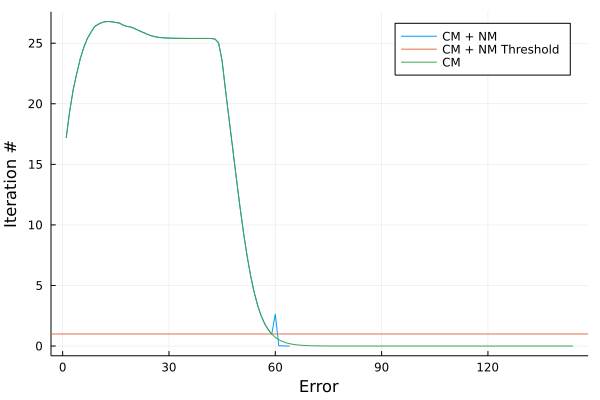
\includegraphics[scale=.75]{question_1.png}

\pagebreak

\section*{Question 2 - GMM First Stage}

The first stage of the GMM estimation uses the 2SLS weighting matrix.  The objective is minimized at $\lambda_p = 0.619$ where the objective function equals 234.76.

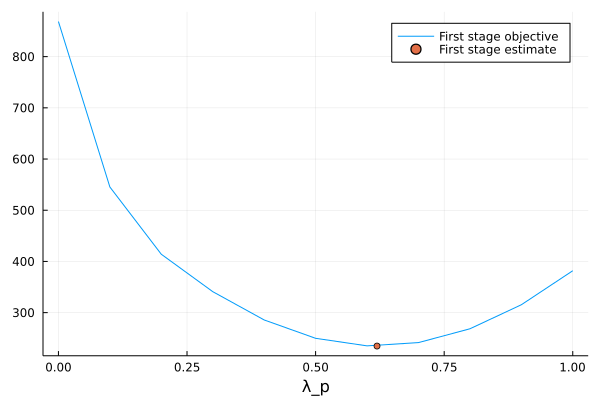
\includegraphics[scale=.75]{question_2.png}

\pagebreak

\section*{Question 3 - GMM Second Stage}

The second stage of the GMM estimation uses weighting matrix based on the first stage estimate.  The objective is minimized at $\lambda_p = 0.564$ where the objective function equals 163.85.

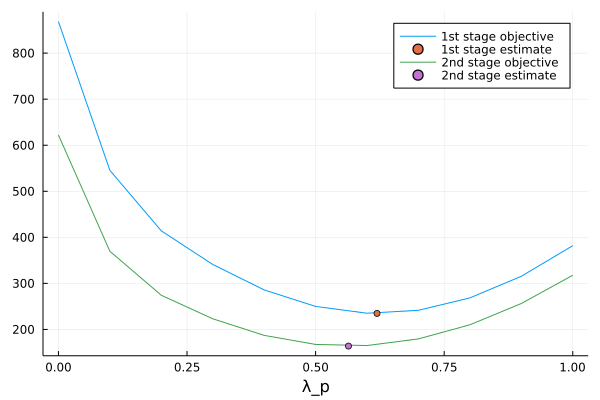
\includegraphics[scale=.75]{question_3.png}

\end{document}

